%
% 2010.01.24 情報システム工学科対応
% 2018.01.05 電子・情報工学科対応
%
\documentclass[10pt]{tpu-abst}
\usepackage[dvipdfmx]{graphicx}
\usepackage{listings,jlisting}

\lstset{language=C,%
    basicstyle={\ttfamily\footnotesize}, %書体の指定
    frame= tb, %フレームの指定
    framesep=5pt, %フレームと中身(コード)の間隔
    breaklines=true, %行が長くなった場合の改行
    linewidth=8cm, %フレームの横幅
    lineskip=-0.5ex, %行間の調整
    tabsize=2 %Tabを何文字幅にするかの指定
	}%
%
% ここでタイトルの設定をします
%
% 自分の名前
\author{尾崎 裕樹}
%
% 学籍番号
\gakuban{1515015}
%
% 研究室の番号
\kouzanum{2}
% 1 情報基盤工学講座 
% 2 情報システム工学講座 
% 3 集積機能デバイス工学講座 
% 4 電子通信システム工学講座 
%
%
% 指導教員名: 
% \kouzaname{ななし} % これはコメントアウトする
% \kouzaname{太田} % 
% \kouzaname{奥原} % 
% \kouzaname{西田} % 
% \kouzaname{榊原} % 
\kouzaname{中村(正)} % 
% \kouzaname{松本(三)} % 
% \kouzaname{唐山} % 
% \kouzaname{鳥山} % 
% \kouzaname{岩本} % 
% \kouzaname{安宅} % 
% \kouzaname{中田} % 
% \kouzaname{浦島} % 
% \kouzaname{松田(敏)} % 
% \kouzaname{岩田} % 
% \kouzaname{松田(弘)} % 
% \kouzaname{石坂} % 
% \kouzaname{三宅} % 
% \kouzaname{小林(香)} % 
% \kouzaname{小島} % 
%
% 発表番号
\happyou{17}
%
% タイトル
\title{プログラミング演習における模範解答を\\用いたテストケース評価基準の自動生成}
%
%----- begin document
%
\begin{document}
%
\maketitle
%
%----- your abstract, please
%

\section{ はじめに}
%
プログラミング演習において,学生自身がテストケースを設計しテストを行うことによって,学生が作成したプログラムを自身で評価することができる。
文献~\cite{a1}では,テストケースが適切であるかを判定する評価基準を用意して,評価基準に対する設計したテストケースの網羅率を求めることでテストケースを評価する手法が提案されている。
このシステムでは,教員が演習問題毎にテストケース評価基準を与える必要がある。

本研究では,テストケース評価基準作成時における教員の負担を減らすために,テストケースの評価基準を自動生成する手法を提案する(図\ref{cap1})。
\begin{figure}[h]
  \centering
  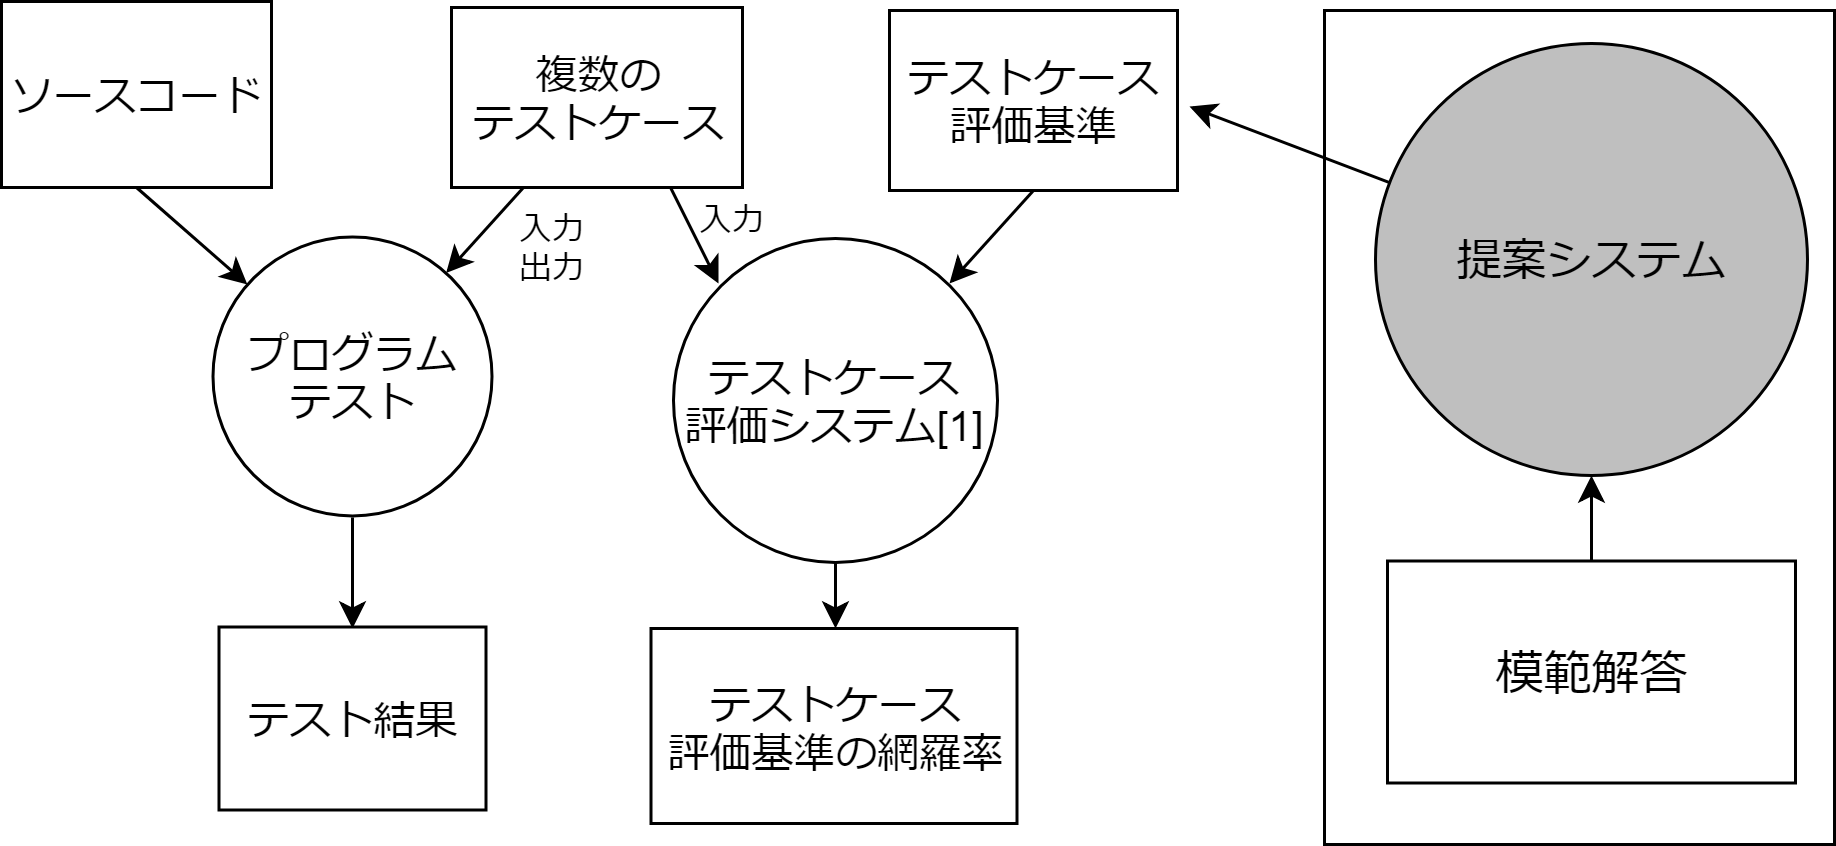
\includegraphics[width=78mm]{提案システムの位置づけ.png}
  \caption{提案システムの位置づけ}
  \label{cap1}
\end{figure}
%
\section{テストケース評価基準の自動生成}
提案システムでは,テストケース評価基準を生成する際に,問題文を分析して記述するのではなく,模範解答のプログラムを解析し,入力がある変数と条件式を抽出することによって,テストケース評価基準を生成する。scanfで2つの整数値を受け取り,大きさを比較した結果を表示するプログラムを例にテストケース評価基準を生成する手順を説明する。

まず,変数宣言部で変数の型と名前を構造体に格納し,標準入力命令部で使用される変数の型に基づきテストケース評価基準を生成する。
\begin{lstlisting}
変数宣言
int num1;
int num2;
標準入力命令
scanf("%d", &num1);
scanf("%d", &num2);

入力のデータ構造
(int num1 int num2)
入力変数から生成されたテストケース評価基準
num1 > 0
num1 == 0
num1 < 0
num2 > 0
num2 == 0
num2 < 0
\end{lstlisting}

次に,条件文を抽出することでテストケース評価基準を生成する。その際ただ抜き出すのではなく,{\tt if else}や{\tt else}の判定をするために,条件文の否定を記述する。 
\begin{lstlisting}
条件文の一部
if (num1 < num2){
	printf("%dより%dの方が大きい。\n", 
		  num1, num2);
}else if (num1 > num2){
	printf("%dより%dの方が大きい。\n",
		  num2, num1);
}else{
	printf("2つの数は同じ値。\n");
}

条件文から生成されたテストケース評価基準
num1 < num2
!(num1 < num2)
num1 > num2
!(num1 > num2)
\end{lstlisting}
% section 3 ----
\section{プログラミング課題への適用}
参考書~\cite{b1}の3章から5章までのサンプルコードや練習問題のうち,標準入力があるプログラムを対象に,作成したシステムによってテストケース評価基準の生成が可能か検証した。
検証を行ったプログラムは26個であり,そのうちの17個で生成可能であった。生成できなかったプログラムはgetcharで入力を行っているプログラムと,同じ変数に複数回入力しているプログラム,switch文や条件演算子で場合分けをしているプログラムであった。

また,6章以降の繰り返しや配列を含むプログラムからはテストケース評価基準の生成ができない。ただし,8章で扱う関数を含むプログラムは入力変数の名前と関数の引数の名前が同じ場合のみ評価基準を生成することが可能である。

% section 4 ----
\section{おわりに}
本研究では,学生が自身でテストケースの評価を行うために用いるテストケース評価基準を自動生成する方法を提案した。
現在対応できていない配列や繰り返し文を含むプログラムからの評価基準の自動生成や,生成した評価基準を入力としてテストケースの評価が可能なシステムの作成が今後の課題である。

\begin{thebibliography}{2}
 \bibitem{a1} {\small 蜂巣吉成,小林悟,吉田敦,阿草清磁: プログラミング演習におけるテストケース評価システム,コンピュータソフトウェア第34巻第4号,2017,pp.54-60}
 \bibitem{b1} {\small 高橋麻奈: やさしいC,SB クリエイティブ,2012}
\end{thebibliography}
%
\end{document}